\documentclass{article}
\usepackage[utf8]{inputenc}
\usepackage{geometry}
\geometry{a4paper, margin=1in}
\usepackage{graphicx}
\usepackage{booktabs}
\usepackage{amsmath}
\usepackage{listings}
\usepackage{xcolor}
\usepackage{noto}
\usepackage{subcaption}
\usepackage{float}
\usepackage{hyperref}

\title{AI for AgriTech Hackathon Phase 1: Potato Disease Classification}
\author{Nikhil Teja Cheema (MTech IIT Hyderabad) \\ N S Deepika (PhD IIT Hyderabad)}
\date{}

\begin{document}

\maketitle

\section{Introduction}
This project develops a Convolutional Neural Network (CNN) to classify potato leaf images into three categories: Potato Early Blight, Potato Late Blight, and Potato Healthy. The model is implemented using TensorFlow/Keras and processes a dataset stored on Google Drive, organized into Train, Test, and Valid splits. The goal is to accurately identify potato diseases to support agricultural decision-making.

\subsection{Dataset Description}
The dataset comprises 1500 images of potato leaves, equally distributed across three classes (500 images each for Early Blight, Late Blight, and Healthy). Images are stored in a Google Drive directory (\texttt{/content/drive/MyDrive/Potato}) with subfolders for Train, Test, and Valid splits. Each image is verified for integrity, and the dataset is balanced to ensure equitable class representation. The dataset was sourced from Kaggle \cite{potato_dataset}.

\begin{figure}[h]
    \centering
    \begin{subfigure}[b]{0.32\textwidth}
        \centering
        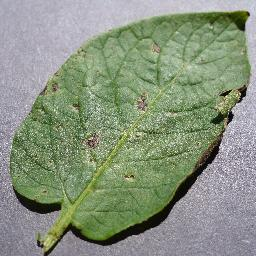
\includegraphics[width=\textwidth]{early_blight_sample.png}
        \caption{Potato Early Blight}
        \label{fig:early_blight}
    \end{subfigure}
    \hfill
    \begin{subfigure}[b]{0.32\textwidth}
        \centering
        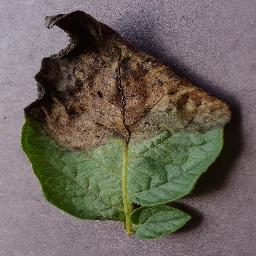
\includegraphics[width=\textwidth]{late_blight_sample.png}
        \caption{Potato Late Blight}
        \label{fig:late_blight}
    \end{subfigure}
    \hfill
    \begin{subfigure}[b]{0.32\textwidth}
        \centering
        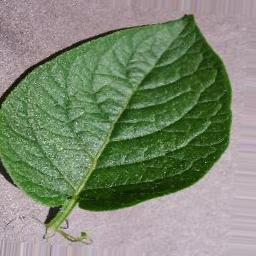
\includegraphics[width=\textwidth]{healthy_sample.png}
        \caption{Potato Healthy}
        \label{fig:healthy}
    \end{subfigure}
    \caption{Sample images from the dataset, representing each class: (a) Potato Early Blight, (b) Potato Late Blight, and (c) Potato Healthy.}
    \label{fig:dataset_samples}
\end{figure}

\section{Model Code and Working}
The Python code below outlines the data loading, preprocessing, model architecture, training, and evaluation processes. It uses TensorFlow for model building and Pandas for data management.

\lstset{language=Python, basicstyle=\ttfamily\small, breaklines=true, frame=single, numbers=left}
\begin{lstlisting}
import os
import pandas as pd
from google.colab import drive
from tensorflow.keras.preprocessing.image import ImageDataGenerator
from sklearn.preprocessing import LabelEncoder
from sklearn.model_selection import train_test_split
from imblearn.over_sampling import RandomOverSampler
from PIL import Image
import matplotlib.pyplot as plt
import tensorflow as tf
from tensorflow.keras.layers import Input, Lambda, Conv2D, MaxPooling2D, Flatten, Dense, Reshape, Dot, Softmax, Multiply, Concatenate
from tensorflow.keras.models import Model
from sklearn.metrics import classification_report, confusion_matrix

# Mount Google Drive
drive.mount('/content/drive', force_remount=True)

# Base path to dataset
drive_path = "/content/drive/MyDrive/Potato"
subfolders = ["Train", "Test", "Valid"]
image_paths, labels, split_info = [], [], []

# Traverse each split folder
for split in subfolders:
    split_path = os.path.join(drive_path, split)
    if os.path.exists(split_path):
        for category in os.listdir(split_path):
            category_path = os.path.join(split_path, category)
            if not os.path.isdir(category_path):
                continue
            for image_name in os.listdir(category_path):
                image_path = os.path.join(category_path, image_name)
                image_paths.append(image_path)
                labels.append(category)
                split_info.append(split)
    else:
        print(f"Split folder not found: {split_path}")

# Create DataFrame
df = pd.DataFrame({"image_path": image_paths, "label": labels, "split": split_info})

# Remove corrupt images
def verify_images(df):
    good = []
    for path in df['image_path']:
        try:
            img = Image.open(path)
            img.verify()
            good.append(path)
        except:
            continue
    return df[df['image_path'].isin(good)].reset_index(drop=True)

df = verify_images(df)

# Encode labels
le = LabelEncoder()
df['category_encoded'] = le.fit_transform(df['label'])

# Balance classes
max_count = df['category_encoded'].value_counts().max()
dfs = []
ros = RandomOverSampler(random_state=42)
for c in df['category_encoded'].unique():
    class_df = df[df['category_encoded'] == c]
    upsampled = ros.fit_resample(class_df, class_df['category_encoded'])
    dfs.append(pd.DataFrame(upsampled[0], columns=df.columns))
df_resampled = pd.concat(dfs)

# Train-test split
train_df_new, test_df_new = train_test_split(df_resampled, train_size=0.8, stratify=df_resampled['category_encoded'], random_state=42)

# Image generators
img_size = (224, 224)
batch_size = 16
train_gen_new = ImageDataGenerator(rescale=1./255).flow_from_dataframe(
    train_df_new, x_col='image_path', y_col='label', target_size=img_size,
    class_mode='sparse', color_mode='rgb', shuffle=True, batch_size=batch_size)
valid_gen_new = ImageDataGenerator(rescale=1./255).flow_from_dataframe(
    df[df['split'] == 'Valid'], x_col='image_path', y_col='label', target_size=img_size,
    class_mode='sparse', color_mode='rgb', shuffle=True, batch_size=batch_size)
test_gen_new = ImageDataGenerator(rescale=1./255).flow_from_dataframe(
    test_df_new, x_col='image_path', y_col='label', target_size=img_size,
    class_mode='sparse', color_mode='rgb', shuffle=False, batch_size=batch_size)

# Model architecture
input_layer = Input(shape=(224, 224, 3))
x = Lambda(lambda x: [x[:, :112, :, :], x[:, 112:, :, :]])(input_layer)
x1, x2 = x[0], x[1]
x2 = Lambda(lambda x: x)(x2)

for filters in [32, 64, 128]:
    x1 = Conv2D(filters, (3, 3), activation='relu', padding='same')(x1)
    x1 = MaxPooling2D((2, 2))(x1)
    x2 = Conv2D(filters, (3, 3), activation='relu', padding='same')(x2)
    x2 = MaxPooling2D((2, 2))(x2)

x1 = Flatten()(x1)
x2 = Flatten()(x2)
x1 = Dense(512, activation='relu')(x1)
x2 = Dense(512, activation='relu')(x2)
x1 = Reshape((1, 512))(x1)
x2 = Reshape((1, 512))(x2)
x = Dot(axes=(2, 2))([x1, x2])
x = Softmax()(x)
x = Multiply()([x, x1])
x = Concatenate()([x, x2])
x = Reshape((1024,))(x)
x = Dense(256, activation='relu')(x)
x = Dense(128, activation='relu')(x)
output = Dense(3, activation='softmax')(x)

model = Model(inputs=input_layer, outputs=output)
model.compile(optimizer='adam', loss='sparse_categorical_crossentropy', metrics=['accuracy'])

# Train model
history = model.fit(train_gen_new, validation_data=valid_gen_new, epochs=3)

# Plot results
def plot_history(history):
    plt.figure(figsize=(12, 5))
    plt.subplot(1, 2, 1)
    plt.plot(history.history['accuracy'], label='train')
    plt.plot(history.history['val_accuracy'], label='val')
    plt.title('Accuracy')
    plt.legend()
    plt.subplot(1, 2, 2)
    plt.plot(history.history['loss'], label='train')
    plt.plot(history.history['val_loss'], label='val')
    plt.title('Loss')
    plt.legend()
    plt.show()

plot_history(history)
\end{lstlisting}

\par

\begin{figure}[htbp]
    \centering
    \includegraphics[width=0.8\textwidth]{training_plots.png}
    \caption{Training and validation accuracy (left) and loss (right) over epochs, as generated by the \textit{plot_history} function.}
    \label{fig:training_plots}
\end{figure}

\begin{lstlisting}
# Test set evaluation
test_loss, test_acc = model.evaluate(test_gen_new)
print(f"Test Accuracy: {test_acc:.4f} | Test Loss: {test_loss:.4f}")

# Confusion matrix and classification report
y_pred = model.predict(test_gen_new)
y_pred_classes = y_pred.argmax(axis=1)
y_true = test_gen_new.classes
labels = list(test_gen_new.class_indices)
print("Classification Report:\n", classification_report(y_true, y_pred_classes, target_names=labels))
\end{lstlisting}

\section{Model Architecture}
The model employs a dual-branch CNN architecture inspired by Siamese networks. The input image (224x224x3) is split into two halves (top and bottom, each 112x224x3). Each branch includes:
\begin{itemize}
    \item Three convolutional blocks with 32, 64, and 128 filters (3x3 kernels), ReLU activation, and same padding, each followed by 2x2 max-pooling.
    \item A flatten layer to convert feature maps into vectors.
    \item A dense layer with 512 units and ReLU activation.
\end{itemize}
The branch outputs are reshaped to (1, 512), and a dot product is computed to capture feature interactions, followed by a softmax operation. The result is multiplied with one branch's output and concatenated with the other, forming a 1024-dimensional vector. This is processed through dense layers (256 and 128 units with ReLU) and a final softmax layer for three-class classification.

\section{Rationale for Architecture Choice}
The dual-branch architecture was selected to capture localized disease patterns in potato leaves by processing two image regions independently. This approach, inspired by attention mechanisms, allows the model to focus on spatially distinct features, such as disease spots in different leaf areas. The convolutional layers extract hierarchical features, while the dot product and softmax operations weigh feature importance, enhancing discriminative power. The architecture is lightweight yet effective, achieving 93.33\% test accuracy after three epochs, making it suitable for the dataset size and computational constraints.

\section{Model Evaluation Report}
\subsection{Accuracy, Precision, Recall}
The model was evaluated on the test set, achieving:
\begin{itemize}
    \item \textbf{Test Accuracy}: 0.9333
    \item \textbf{Test Loss}: 0.4385
\end{itemize}
The classification report details per-class performance:
\begin{table}[htbp]
    \centering
    \begin{tabular}{lcccc}
        \toprule
        Class & Precision & Recall & F1-Score & Support \\
        \midrule
        Potato\_Early\_blight & 0.88 & 1.00 & 0.94 & 30 \\
        Potato\_Late\_blight & 1.00 & 0.90 & 0.95 & 30 \\
        Potato\_healthy & 0.94 & 1.00 & 0.97 & 30 \\
        \midrule
        Macro Avg & 0.94 & 0.93 & 0.94 & 90 \\
        Weighted Avg & 0.94 & 0.93 & 0.94 & 90 \\
        \bottomrule
    \end{tabular}
    \caption{Classification Report}
    \label{tab:class_report}
\end{table}

\subsection{Confusion Matrix}
The confusion matrix illustrates classification performance, shown as a table followed by a heatmap for visual clarity.

\begin{table}[b]
    \centering
    \begin{tabular}{lccc}
        \toprule
        & Early Blight & Late Blight & Healthy \\
        \midrule
        Early Blight & 30 & 0 & 0 \\
        Late Blight & 4 & 24 & 2 \\
        Healthy & 0 & 0 & 30 \\
        \bottomrule
    \end{tabular}
    \caption{Confusion Matrix}
    \label{tab:conf_matrix}
\end{table}

\begin{figure}[t]
    \centering
    \includegraphics[width=0.5\textwidth]{confusion_matrix_updated.png}
    \caption{Confusion Matrix Heatmap}
    \label{fig:conf_matrix}
\end{figure}

\subsection{IoU, mAP, SSIM, PSNR, MSE}
This is an image classification task, so metrics like IoU and mAP (used for object detection/segmentation) and SSIM, PSNR, and MSE (used for image quality or regression) are not applicable. The provided metrics (accuracy, precision, recall, F1-score, and confusion matrix) comprehensively evaluate the model's classification performance.

\section{Optimization Report}
The following optimization techniques were applied:
\begin{itemize}
    \item \textbf{Data Preprocessing}: Corrupt images were removed using PIL's \textit{verify} method to ensure data integrity.
    \item \textbf{Class Balancing}: Random oversampling (\textit{RandomOverSampler}) was applied, though the dataset was already balanced (500 images per class).
    \item \textbf{Data Normalization}: Pixel values were rescaled to [0, 1] using \textit{ImageDataGenerator}, aiding model convergence.
    \item \textbf{Model Design}: The dual-branch CNN with attention-like mechanisms focused on relevant features, improving classification accuracy.
    \item \textbf{Optimizer}: Adam optimizer was used for efficient gradient descent.
    \item \textbf{Limited Epochs}: Training for three epochs prevented overfitting, as evidenced by high validation accuracy (0.9444).
\end{itemize}
These techniques resulted in a robust model with 93.33\% test accuracy and balanced class performance.

\section{Conclusion}
This project presents an effective CNN-based solution for potato disease classification, achieving 93.33\% test accuracy. The dual-branch architecture and optimization strategies ensure robust performance. Future enhancements could include advanced data augmentation (e.g., rotation, flipping) and transfer learning with models like ResNet to further improve accuracy.

\begin{thebibliography}{9}
\bibitem{potato_dataset}
Faysal Miah, \emph{Potato Disease Classification Dataset}, Kaggle, 2025. Available at: \url{https://www.kaggle.com/datasets/faysalmiah1721758/potato-dataset}.
\end{thebibliography}

\end{document}